\section{Theoretical Analysis}
\label{sec:analysis}

In this section, the circuit shown in Figure~\ref{fig:T2Circuit} is analysed theoretically in six steps.

In step (1), first of all, we used the nodal method to determine the voltages in all nodes and currents in all branches for t<0. The results are shown in Table~\ref{tab:TA1}.

\begin{table}[h]
  \centering
  \begin{tabular}{|l|r|}
    \hline    
    {\bf Nodes and branches} & {\bf Value [V]/[A]} \\ \hline
    v1 & 5.134164 \\ \hline
v2 & 4.929601 \\ \hline
v3 & 4.510168 \\ \hline
v4 & 0.000000 \\ \hline
v5 & 4.957651 \\ \hline
v6 & 5.588276 \\ \hline
v7 & -2.095712 \\ \hline
v8 & -3.151534 \\ \hline
  \end{tabular}
  \caption{Theoretical voltage values for each node, expressed in Volt, and current values for each branch, expressed in Ampere.}
  \label{tab:TA1}
\end{table}

After this, in step (2), we determined the equivalent resistance as seen from the capacitor terminals. In order to do so, we followed the professor's sugestion. Therefore, in this section of the analysis, the capacitor was replaced by a voltage source Vx. Ix and Vx were calculated using Octave. After this, the value of the equivalent resistance was computed and determined. These procedures were necessary because they allowed us to calculate the time constant (\tau) without which we would no be able to performe all the theoretical analisys in the following sections. 

\begin{equation}
  \tau = R_{eq}C,
  \label{eq:tau}
\end{equation}


The computed results can be found in Table~\ref{tab:TA2}.

\begin{table}[h]
  \centering
  \begin{tabular}{|l|r|}
    \hline    
    {\bf Computed Results} & {\bf Values} \\ \hline
    v1 & 0.000000 \\ \hline
v2 & 0.000000 \\ \hline
v3 & 0.000000 \\ \hline
v4 & 0.000000 \\ \hline
v5 & 0.000000 \\ \hline
v6 & 8.739810 \\ \hline
v7 & 0.000000 \\ \hline
v8 & 0.000000 \\ \hline
Ix & -0.002826 \\ \hline
Vx & 8.739810 \\ \hline
Req & -3092.796241 \\ \hline
  \end{tabular}
  \caption{Computed results: voltage expressed in Volt, current in Ampere and resistence in Ohm.}
  \label{tab:TA2}
\end{table}

Later, in step (3), we used the value of the equivalent resistant calculated in point (2) to find the natural solution of v6. Knowing that "\tau" is calculated by the equation~\ref{tau}, in Equation~\ref{eq:natsol} we find the formula required to calculate the natural solution we wanted. 

\begin{equation}
  V_{6n}(t) = V_{x}e^{-\frac{t}{\tau}},
  \label{eq:natsol}
\end{equation}

Also the solution is ploted in Figure~\ref{figure:plotA(4)} where the x-axis corresponds to time, t, expressed in [ms] and the y-axis corresponds to the natural solution of v6, 'v6n', expressed in [V].

\begin{figure}[h] \centering
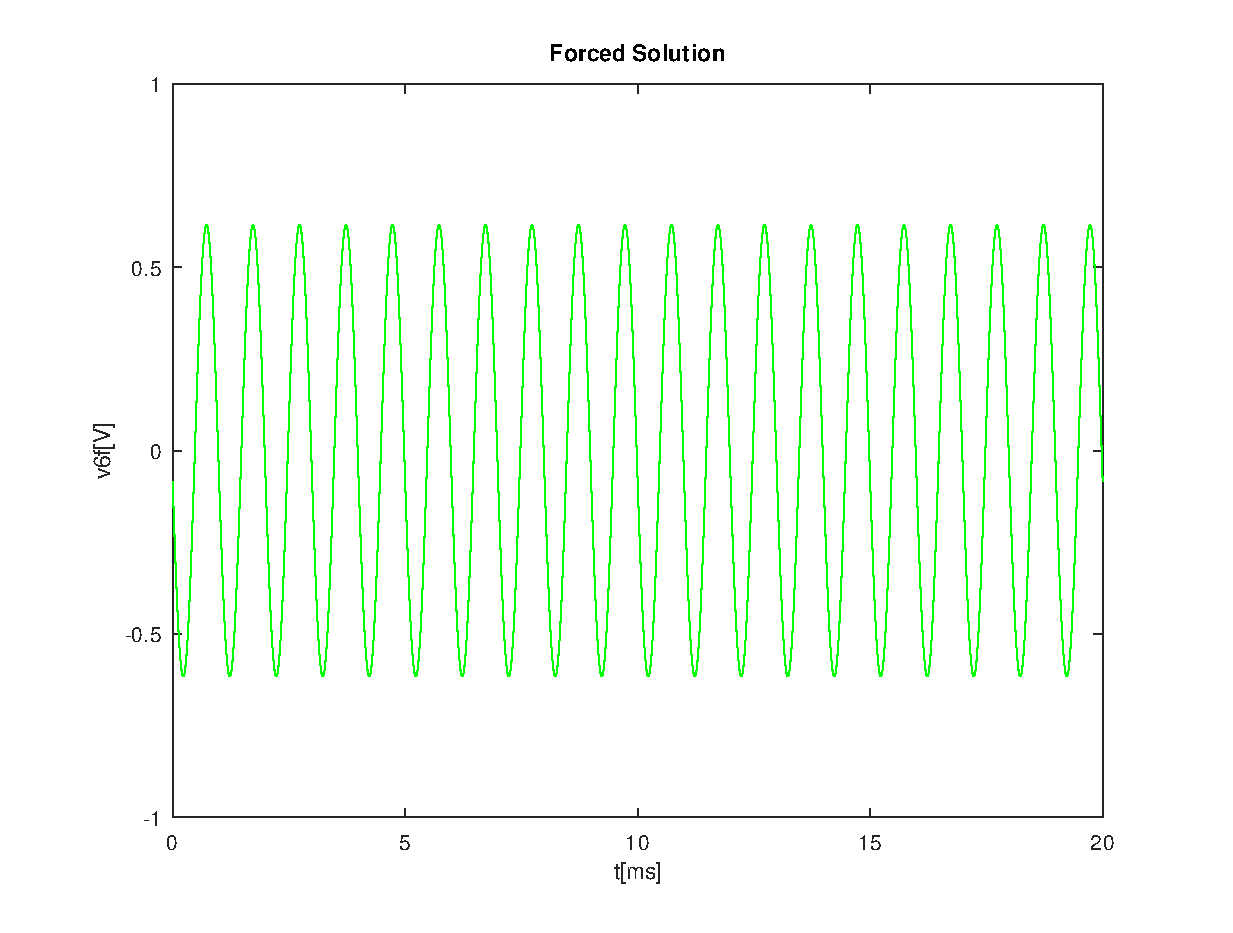
\includegraphics[width=0.8\linewidth]{forced_solution.eps}
\caption{Plot of v6n(t) in the interval [0, 20]ms.}
\label{fig:plotA(4)}
\end{figure}

In step (4), the forced solution v6f(t) was determined for f=1KHz and for t in the interval [0,20]ms. Moreover, the capacitance was replaced by the impedance, 'Z', and Vs was considered equal to one. The complex amplitudes in the nodes are shown in Table~\ref{tab:TA4}.

\begin{table}[h]
  \centering
  \begin{tabular}{|l|r|}
    \hline    
    {\bf Nodes} & {\bf Complex Amplitudes} \\ \hline
    |v1| & 1.000000 \\ \hline
|v2| & 0.960156 \\ \hline
|v3| & 0.878462 \\ \hline
|v4| & 0.000000 \\ \hline
|v5| & 0.965620 \\ \hline
|v6| & -0.609606 \\ \hline
|v7| & -0.408190 \\ \hline
|v8| & -0.613836 \\ \hline
  \end{tabular}
  \caption{Complex amplitudes in the nodes, expressed in Volt.}
  \label{tab:TA4}
\end{table}

Then, in step (5), we determined the final total solution v6(t) by converting the phasors to real time functions for f=1KHz, and superimposing the natural and forced solutions, just like it was asked by the professor. In Figure~\ref{fig:plotA(5)} are plotted both vs(t) and v6(t) in the interval [-5, 20]ms.

\begin{figure}[h] \centering
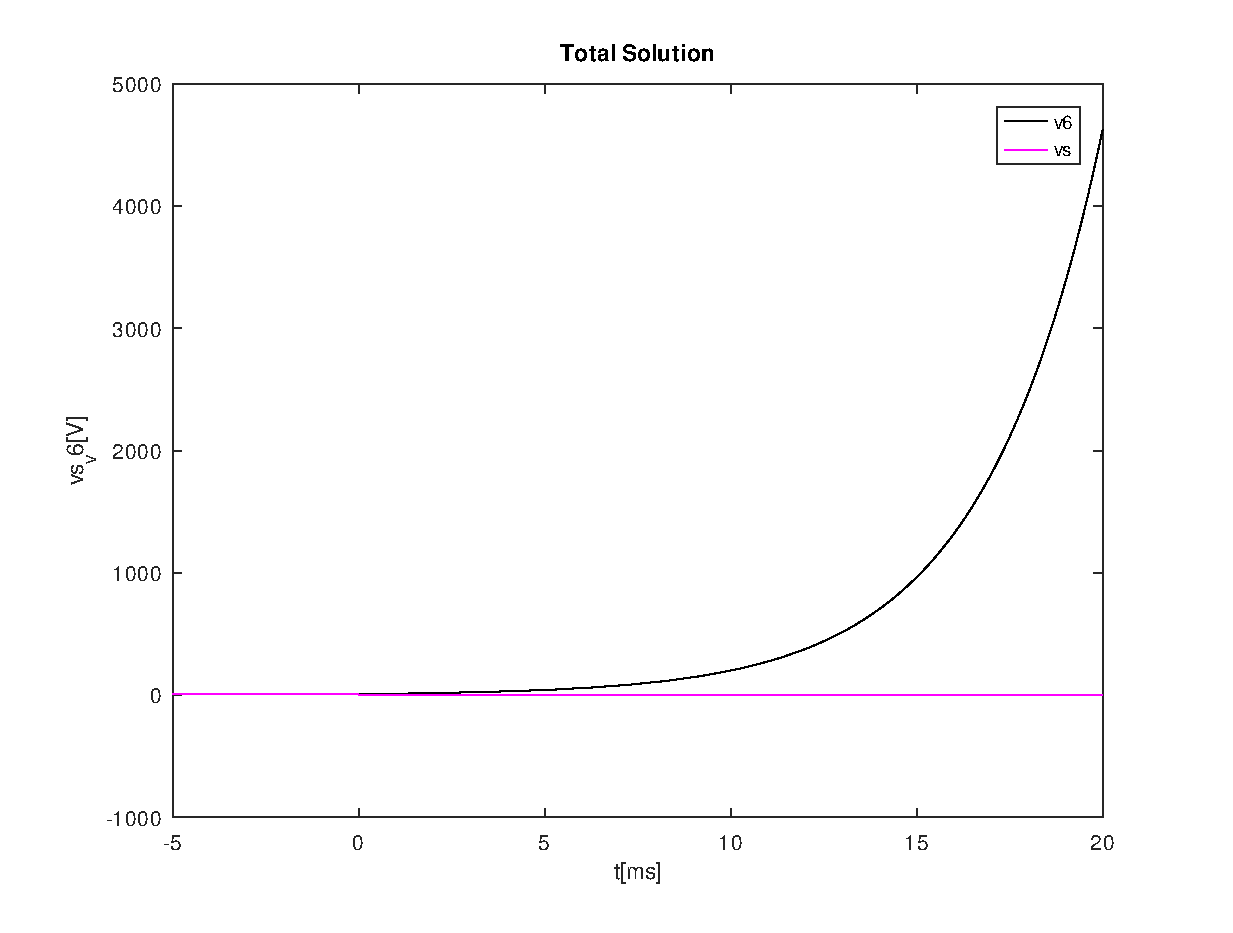
\includegraphics[width=0.8\linewidth]{Total_Solution.eps}
\caption{Plot of v6(t) and vs(t) in the interval [-5, 20]ms.}
\label{fig:plotA(5)}
\end{figure}

Finally, in step (6), we calculted the frequency responses vc(f) and v6(f) for frequency in the interval [0.1, 1M]Hz. The functions vs(f), vc(f) and v6(f) are represented in two plots: one of amplitude frequency response, represented in Figure~\ref{fig:plotA(61)} and the other of phase response, shown in Figure~\ref{fig:plotA(62)}. Note that in both graphs, frequency logscale magnitude is in dB and phase in degrees.

\begin{figure}[h] \centering
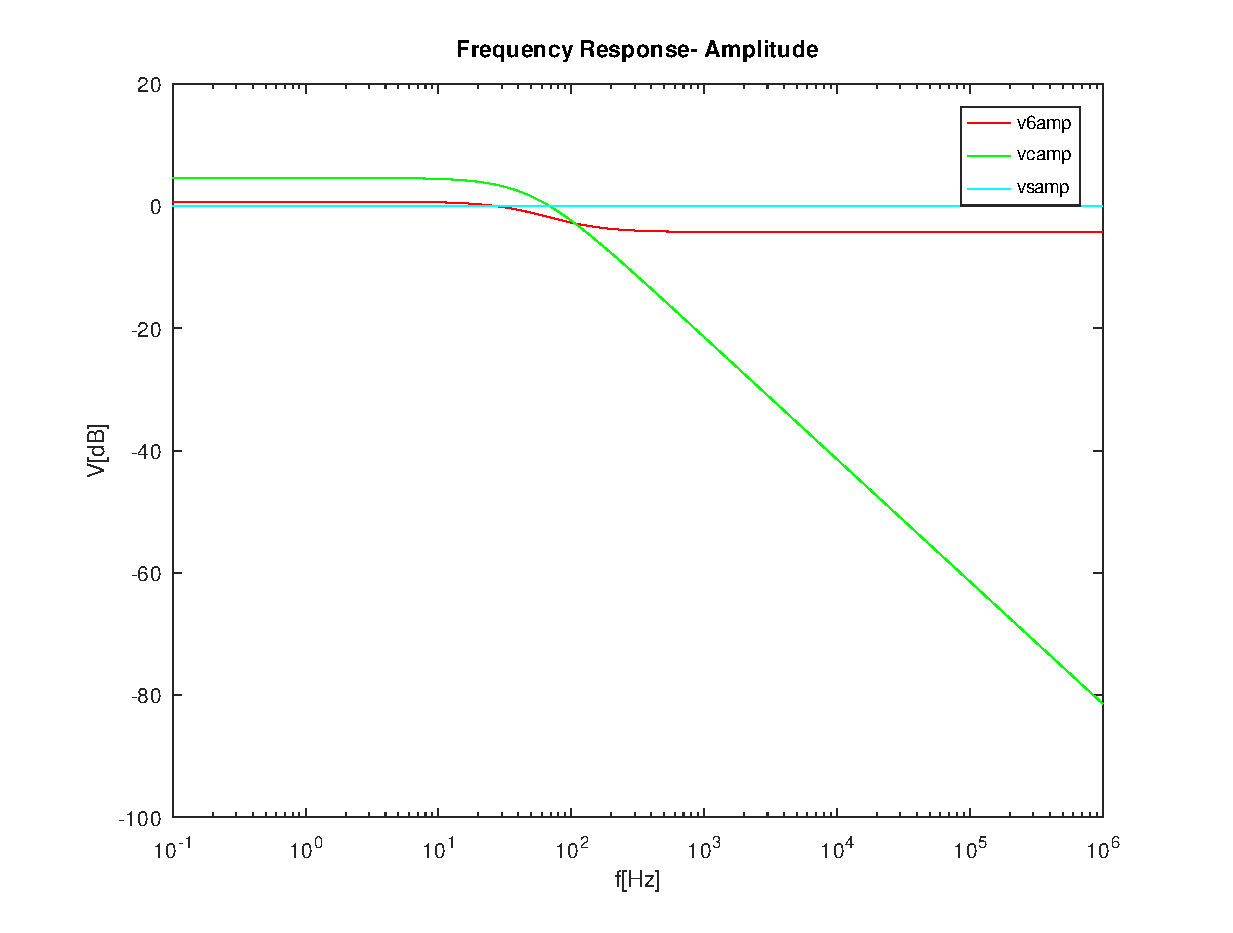
\includegraphics[width=0.8\linewidth]{Frequency_Response_Amplitude.eps}
\caption{Plot of amplitude frequency response (for vs(f), vc(f) and v6(f)) in the interval [0.1, 1M]Hz.}
\label{fig:plotA(61)}
\end{figure}

\begin{figure}[h] \centering
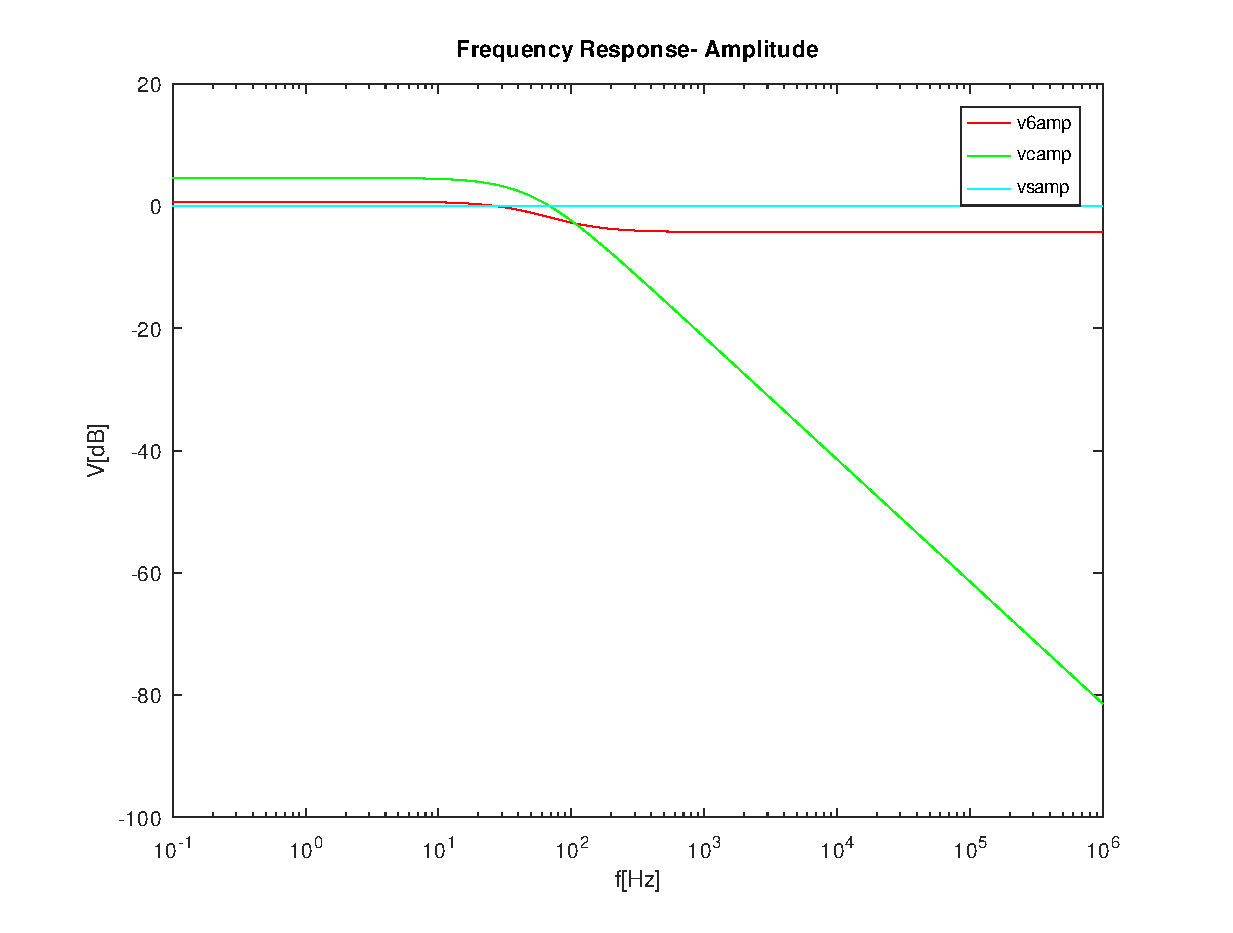
\includegraphics[width=0.8\linewidth]{Frequency_Response_Phase.eps}
\caption{Plot of phase response (for vs(f), vc(f) and v6(f)) in the interval [0.1, 1M]Hz.}
\label{fig:plotA(62)}
\end{figure}

How and why they differ??....
